%% LaTeX2e class for seminar theses
%% seminar.tex
%% 
%% Karlsruhe Institute of Technology

%%
%%
%% Version 1.0.3, 2020-06-26

%% Available page modes: oneside, twoside
%% Available languages: english, ngerman
%% Available modes: draft, final (see README)
\documentclass[twoside, english]{sdqseminar}

%% ---------------------------------
%% | Information about the thesis  |
%% ---------------------------------

%% Name of the author
\author{Chen Shao}

%% Title (and possibly subtitle) of the thesis
\title{Multi-View Depth Estimation}

%% Type of the thesis 
% \thesistype{Seminar Thesis}

%% Change the institute here, ``IPD'' is default
% \myinstitute{Institute for \dots}

%% The advisors are PhD Students or Postdocs
\advisor{M.Sc. Fabian Duffhaus}

\settitle

%% --------------------------------
%% | Settings for word separation |
%% --------------------------------

%% Describe separation hints here.
%% For more details, see 
%% http://en.wikibooks.org/wiki/LaTeX/Text_Formatting#Hyphenation
\hyphenation{
% me-ta-mo-del
}

%% --------------------------------
%% | Bibliography                 |
%% --------------------------------

%% Use biber instead of BibTeX, see README
\usepackage[citestyle=numeric,style=numeric,backend=biber]{biblatex}
\addbibresource{seminar.bib}

%% ====================================
%% ====================================
%% ||                                ||
%% || Beginning of the main document ||
%% ||                                ||
%% ====================================
%% ====================================
\begin{document}

%% Set PDF metadata
\setpdf

%% Set the title
\maketitle

%% ----------------
%% |   Abstract   |
%% ----------------
 
%% The text is included from the following files:
%% - sections/abstract

\begin{abstract}
%% LaTeX2e class for seminar theses
%% sections/abstract_en.tex
%% 
%% Karlsruhe Institute of Technology
%% Institute for Program Structures and Data Organization
%% Chair for Software Design and Quality (SDQ)
%%
%% Dr.-Ing. Erik Burger
%% burger@kit.edu
%%
%% Version 1.0.2, 2020-05-07

English abstract.
\end{abstract}

%% -----------------
%% |   Main part   |
%% -----------------
%% LaTeX2e class for seminar theses
%% sections/content.tex
%% 
%% Karlsruhe Institute of Technology
%% Institute for Program Structures and Data Organization
%% Chair for Software Design and Quality (SDQ)
%%
%% Dr.-Ing. Erik Burger
%% burger@kit.edu
%%
%% Version 1.0.2, 2020-05-07

\section{Basic of camera geometry}
\label{ch:basic of camera geometry}

%% -------------------
%% | Example content |
%% -------------------
The first generation of stereo-based depth estimation methods relied typically on matching pixels across multiple images captured using accurately calibrated cameras. Although these techniques can achieve good results, they are still limited in many aspects. For instance, they are not suitable when dealing with occlusions, featureless regions, or highly textured regions with repetitive patterns. We will introduce the camera geometric relationship, conventional pixel matching method and some important concept in multi-view estimation. e.g. disparity and depth. 

\subsection{camera model: projection matrix}
\label{projection matrix}
A test object introduces a characteristic modulation to the irradiated light, so that one can obtain information about the test object from the emitted light\cite{1400121}. This interactive effect can be described as simplified model called light filed $\mathcal{L}(x_{w}, \beta)$, where the process of radiance of all light rays coming from a point $x_{w}$ of the test object in the direction $\beta$ is modelled. The light field $\mathcal{L}(x_{w}, \beta)$ is a five-dimensional function of the position $x_w = (x_w, y_w, z_w)$, $T \in \mathrm{R}_3$ and the direction $\beta = (\beta_1, \beta_2)$. If $\mathcal{L}(x_{w}, \beta)$ is known for all of the surface’s points $x_w \in \mathrm{SF}$, then the light field $\mathcal{L}(x_{w}, \beta)$, $u \in \mathrm{R}_3$ induced by the test object is uniquely defined for the surrounding space. In our project, we used a completely simplified model based on the lifht field model, which has only four parameters, namly $\mathcal{L}(x_{w}, o_i, \lambda)$, where $o_i$ defines the angular information of the camera in three dimensional world and $\lambda$ represents the color perception through the microlens, in this situation $\lambda = (l_r, l_g, l_b)$. To explain this model intuitively we introduce the pinhole camera model and derive the projection matrix of a normal camera. 
\begin{equation}
\label{eqn:lf_model1}
    \mathcal{L}(x_{w}, o_i, \lambda) \quad x_w=(x_x, x_y,x_z), \quad o_1 = (o_x, o_y, o_z), \quad \lambda = (l_r,l_g,l_b)
\end{equation}

\begin{figure}
\centering
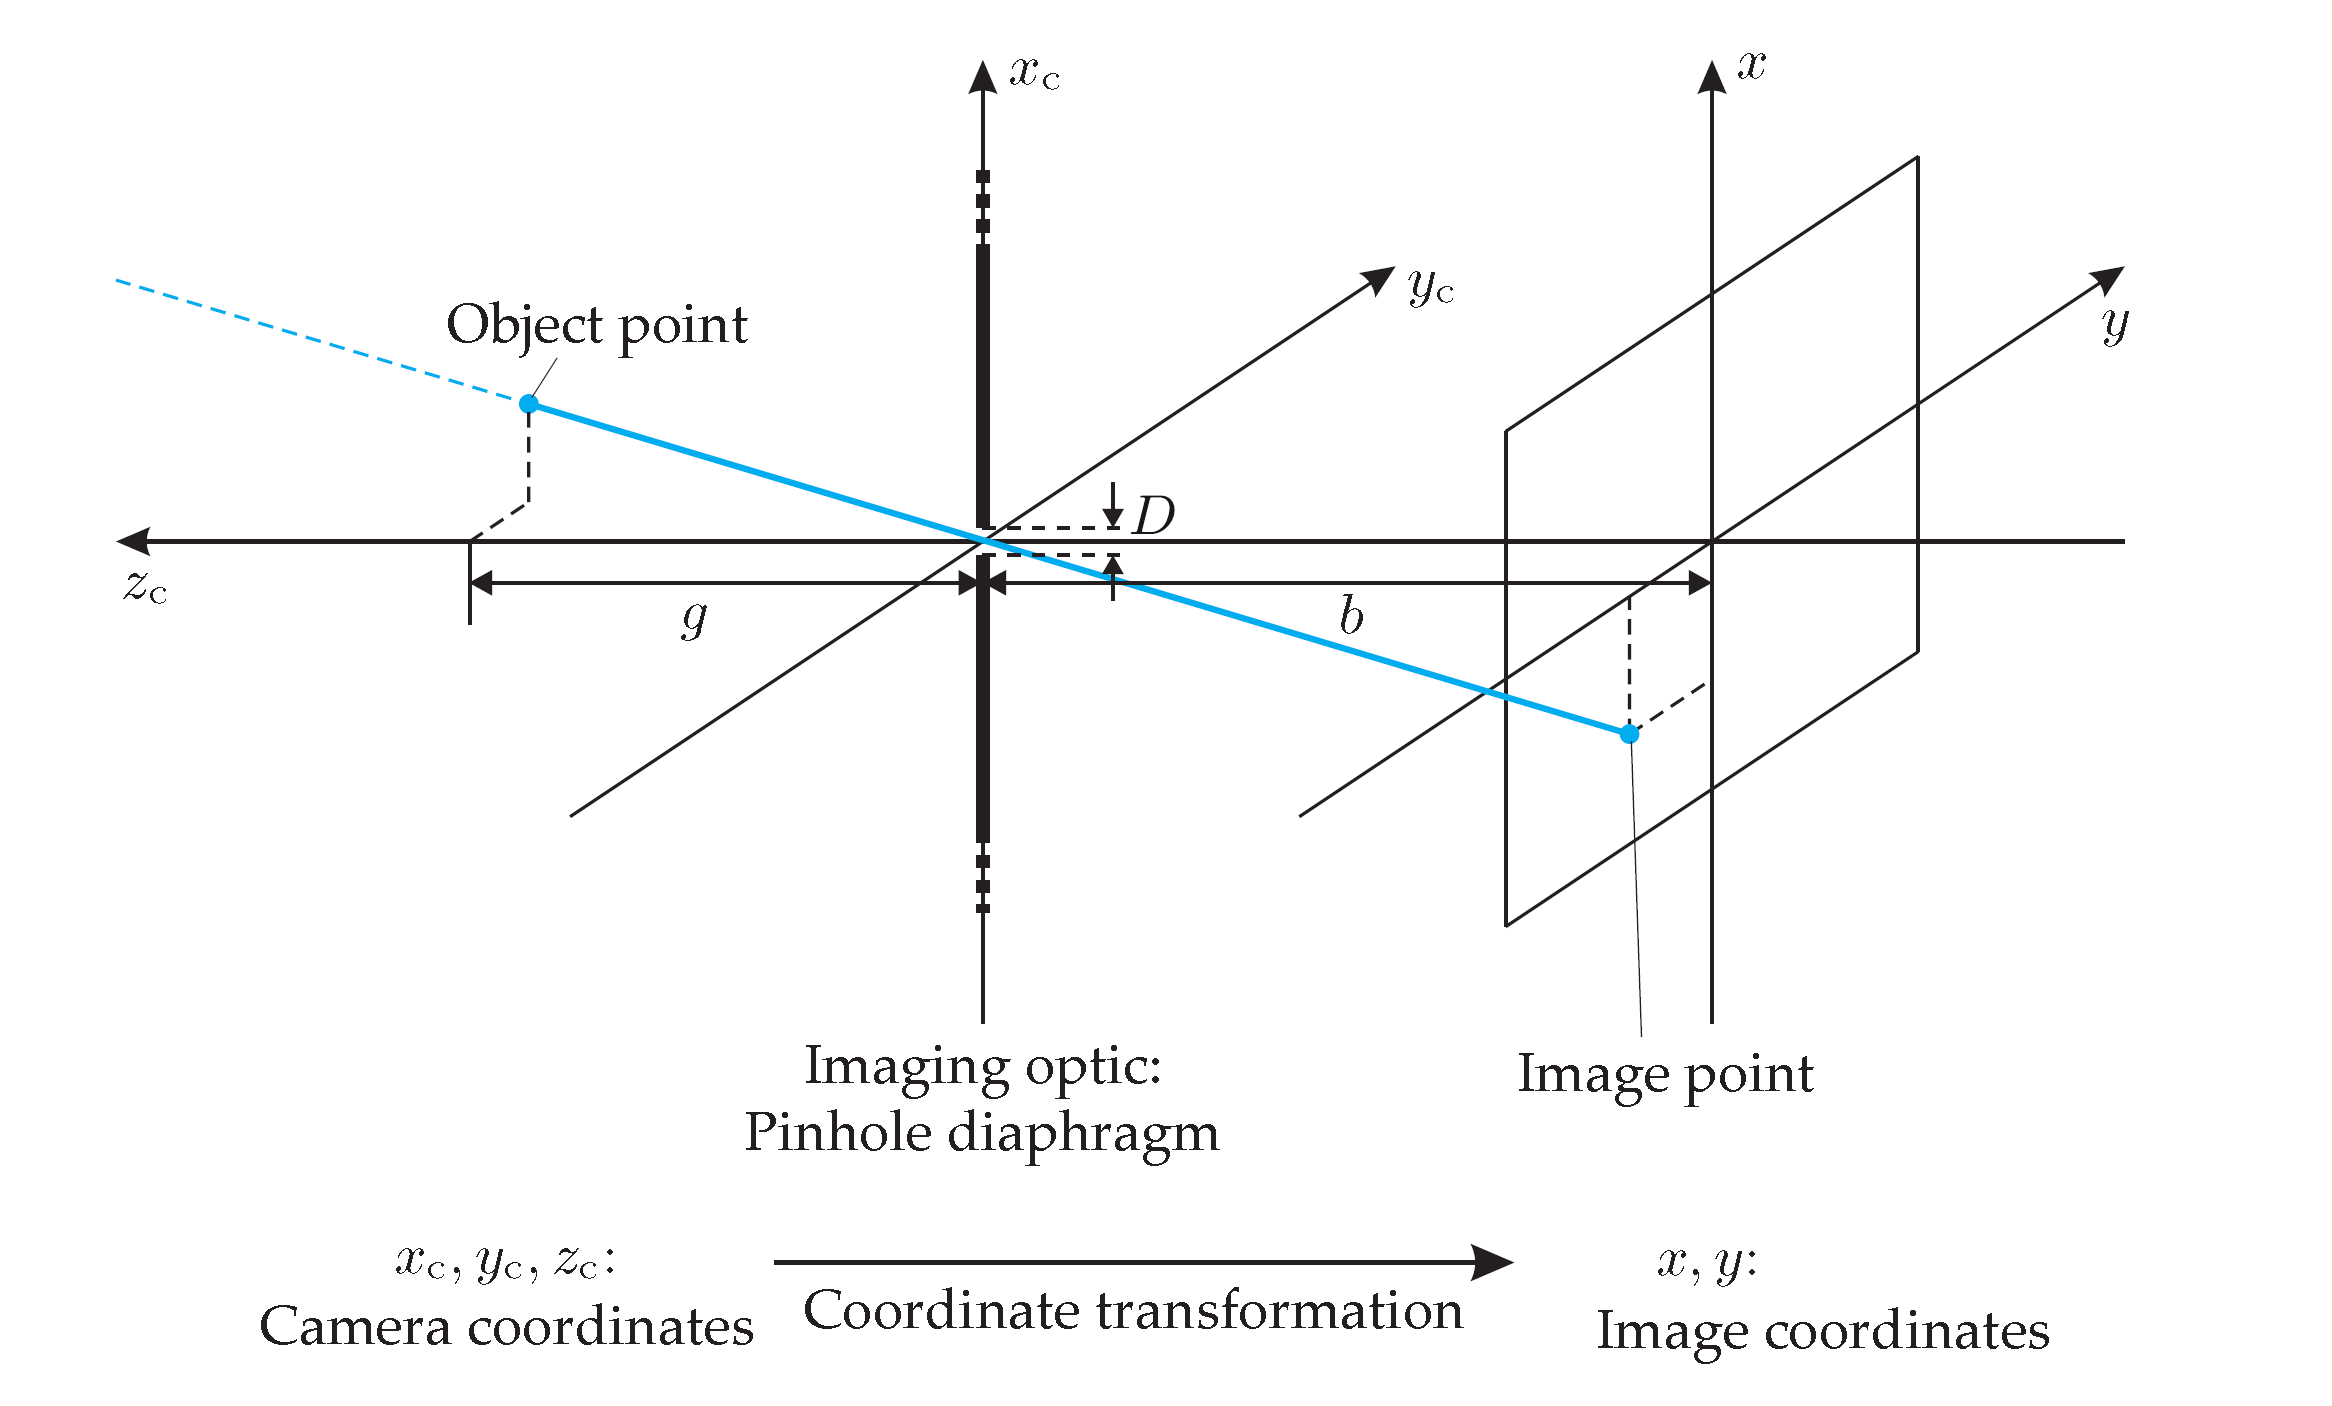
\includegraphics[width=15cm]{images/camera_model.PNG}
\caption{pinhole camera model}
\label{fig:pinhole camera model}
\end{figure}

Before the actual camera model will be explained, we extend the model $x_w$ in \ref{eqn:lf_model1} appropriately. We denote some concept and explain it using the example of pinhole camera. Firstly we denote world coordinate system as $(x_w)$, which defines the position of each object point. The information in this three dimensional world coordinate will be acquisited and imaged in the three dimensional camera coordinate. The transformation from world coordinates to camera coordinates is equivalent to a linear mapping, which can be expressed by a combination of rotation and a subsequent translation transformation:
\begin{equation}
\label{eqn:world-camera transformation}
\begin{pmatrix}
x_c \\
y_c\\
z_c
\end{pmatrix} = \mathrm{R}
\begin{pmatrix}
x_w \\
y_w\\
z_w
\end{pmatrix} + \mathrm{t}
\end{equation}
where $t \in \mathbb{R}_3$ is the translation vector and $\mathbb{R} ∈ \mathbb{R}_{3\times3}$ an orthogonal rotation matrix. Each camera can be characterised as two intrinsic matrices. $\mathrm{C} = [\mathrm{R}\,|\,\mathrm{T}]$.
Until now, the imaging process is still well-defined, unfortunately depth information will be lost when it projected onto image plane, which denoted as $(i_x, i_y)$. Here we just discuss this ill-posed projection process to make the principle clear. The actual camera in the real world can have more completed acquisition process. The distance between the aperture and the image plane is called the image distance $b$. In the case of pinhole camera (Figure \ref{fig:pinhole camera model}), the optical mapping of an object point $x_c$ to an image point $x$ can be mathematically as following:
\begin{equation}
\label{eqn:camera-image transformation}
\begin{pmatrix}
x\\
y\\
\end{pmatrix} = \mathrm{\frac{b}{z_c}}
\begin{pmatrix}
x_c \\
y_c
\end{pmatrix}
\end{equation}
Until now we have introduced the image acquisition process using a simple example. Reconstruct the depth map using integrated light field is a ill-posed problem but not absolutely unsolvable. 





% \subsection{Example: Tables}
% \label{sec:Introduction:Tables}
% \begin{table}
% \centering
% \begin{tabular}{r l}
% \toprule
% abc & def\\
% ghi & jkl\\
% \midrule
% 123 & 456\\
% 789 & 0AB\\
% \bottomrule
% \end{tabular}
% \caption{A table}
% \label{tab:atable}
% \end{table}
\subsection{Disparity and depth estimation}
\label{disparity and depth estimation}

In last section we introduced the theory of imaging process. Depth estimation with single image is without prior knowledge theoretically not possible. An intuitive interpretation for this can be explained through the humanly imaging system. People can not identify the depth and the position of the object using just one eye. This section will introduce the method to estimation the depth using double images. 

In the case of the multi-view images the depth is estimated through the disparity. Mathematically it can be the depth of each pixel well determined by disparity of each, which can be directly derived through geometrical method. We assume that two cameras located at the baseline which is parallel with the optic axis and share the same intrinsic parameter, e.g focal length (Figure \ref{fig:disparity}). Disparity of a given pixel in the image coordinate, denoted as $d$ is defined as the distance moving from left to right view in images, in case of the given Figure  \ref{fig:disparity} is $d=x_1-x_2$. 
Afterwards the depth denoted as $z$ can be derived as following,
where $f$, $x1$, $x_2$, $b$ are given, according to the principle of similar triangles we get:

\begin{figure}
\centering
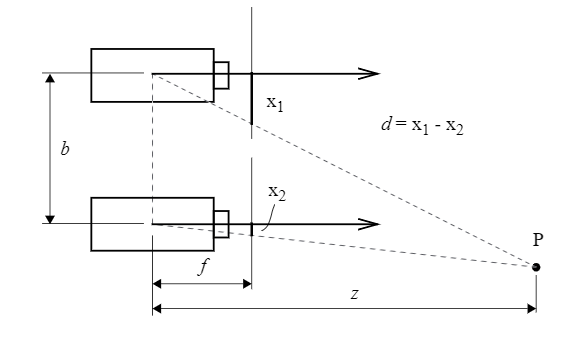
\includegraphics[width=15cm]{images/disparity.PNG}
\caption{disparity of multi-view images system}
\label{fig:disparity}
\end{figure}

\begin{gather}
\label{}
    \frac{z}{f} =  \frac{x}{x_1} \\
    \frac{z}{f} =  \frac{x-b}{x_2}
\end{gather}
where the variable $x$ defines the object's position in the world coordinate in x axis, that is unknown but determined. We solve it for variable $x$ and get: 
\begin{equation}
    x = \frac{b*x_l}{x_l-x_r}
\end{equation}
Finally we get the expression of the depth $z$ with respect to $d$, $f$, $d$.
\begin{equation}
    z = \frac{f*b}{x_l-x_r} = \frac{f*b}{d}
\end{equation}
So far, we have taken the mapping relationship between the disparity and depth. Therefore, the stereo-based depth estimation
methods relied typically on matching pixels across multiple images captured using accurately calibrated cameras. 

\subsection{overview: first and second generation methods}
\label{overview: first and second generation methods}
In section \ref{disparity and depth estimation} we know that the depth estimation relys on the calculation of the disparity. Actually the first generation of stereo-based depth estimation methods relied typically on matching pixels across multiple images captured using accurately calibrated cameras. Although these techniques can achieve good results, they are still limited in many aspects. Those first generation methods distinguish between four steps that most stereo methods perform, i.e. matching cost computation, cost aggregation, disparity computation/optimization and disparity
refinement\cite{scharstein2002taxonomy}. We will introduce the the BM, SGM, SGBM and GC successively. Understanding these traditional methods give aid to have a basic understanding of existing algorithms, that do not rely on match learning. Futhermore, it can also help us to design an appropriate machine learning algorithms to estimate depth maps. 

The goal of a stereo correspondence algorithm is then to produce a univalued function in disparity space d(x, y) that best describes the shape of the surfaces in the scene. This can be viewed as finding a surface embedded in the disparity space image that has some optimality property, such as lowest cost and best (piecewise) smoothness.

\subsubsection{Basic}
\label{BM Algorithm}
Before more details about the BM will be given, we want to reformulate the problem and introduce the necessary notations for further discussion, assume we want to estimate the disparity of a pixel $(x,y) \in \mathbb{R}\times \mathbb{R}$ between reference image $r$ and  $(x^{'},y^{'}) \in \mathbb{R}\times \mathbb{R}$ matching images $m$ where s = ±1 is a sign chosen so that disparities are always positive. Note that since our images are numbered from leftmost to rightmost, the pixels move from right to left\cite{scharstein2002taxonomy}.
\begin{equation}
    x^{'} = x + sd(x,y), \quad y^{'} = y
\end{equation}
$d(x,y)$ is the epipolar constraint, which helps to decrease the search scope. From this point of view there are two mutually exclusive strategies to search for disparity. local (window-based) algorithms, where the disparity computation at a given point depends only on intensity values within a finite window, usually make implicit smoothness assumptions by aggregating support. This kind of methods can be broken down into steps:
\begin{enumerate}
    \item the matching cost is the squared difference of intensity values at a given disparity;
    \item aggregation is done by summing matching cost over square windows with constant disparity;
    \item disparities are computed by selecting the minimal (winning) aggregated value at each pixel.
\end{enumerate}
Some useful matching cost function is given here:
\begin{enumerate}
    \item Absolute differences
        \begin{equation}
            e(x,y,d) = |I_R(x,y)-I_T(x+d,y)|
        \end{equation}
    \item Squared differences
        \begin{equation}
            e(x,y,d) = (I_R(x,y)-I_T(x+d,y))^2
        \end{equation}
    \item Robust Matching measures (M-estimators)
    \begin{equation}
        e(x,y,d) = min \{|I_R(x,y)-I_T(x+d,y))|, T \}
    \end{equation}
\end{enumerate}
The matching cost values over all pixels and all disparities form the initial disparity space image $C0(x, y, d)$. Local and window-based methods aggregate the matching cost by summing or averaging over a support region in the DSI  $C(x, y, d)$. Aggregation with a fixed support region can be performed using 2D or 3D convolution, 
\begin{equation}
    C(x, y, d) = w(x, y, d) \ast C_0(x, y, d)
\end{equation}



On the other hand, global algorithms make explicit smoothness assumptions and then solve an optimization problem. Such algorithms typically do not perform an aggregation step, but rather seek a disparity assignment (step 3) that minimizes a global cost function that combines data (step 1) and smoothness terms. The object is to find a disparity function $d$ minimizes a global energy,

\begin{equation}
    E(d) = E_{data}(d) + \lambda E_{smooth}(d)
\end{equation}

\subsubsection{Block Matching}
\label{BM}
Until now, we already have a big image of the traditional methods. Next we will introduce the basic algorithm block matching algorithm. We make a implicit smoothness assumptions, that the disparity within a finite window is smooth. We calculate the summed cost, for example, the traditoinal sum-of-squared-differences (SSD) over all pixels in the left view images using following equation. 
\begin{equation}
    C(x, y, d) = \sum_{x \in \mathbb{R}} (I_R(x, y)-I_T(x+d, y))^2
\end{equation}
Computing the final disparities is trivial: simply choose at each pixel the disparity associated with the minimum cost value. Thus, these methods perform a local “winner-take-all”
(WTA) optimization at each pixel. In other words, choose the smallest value in the disparity space.  
% https://jiweibo.github.io/StereoBM/


\subsubsection{Semi-Global Matching Algorithm}
\label{Semi-Global Matching}
This subsection we introduce one of the most popular algorithms Semi-Global Matching. Semi-Global Matching Algorithm can be formulated as finding the disparity image D that minimizes the energy $E(D)$,which calculates the matching cost hierarchically by Mutual Information. Cost aggregation is performed as approximation of a global energy function by pathwise optimizations from all directions through the image. Disparity computation is done by winner takes all and supported by disparity refinements like consistency checking and sub-pixel interpolation. Multi-baseline matching is handled by fusion of disparities. Further disparity refinements include peak filtering, intensity consistent disparity selection and gap interpolation images and the fusion of several disparity images using orthographic projection\cite{hirschmuller2007stereo}. 

Matching cost calculation in SGM is based on the Mulual Information(MI), which is dependent on the distribution of the pixel but not the pixel itself, so it is insentitvie to recording and illumination changes. The MI's definition is given as
\begin{equation}
    MI_{I_1, I_2} = H_1 + H_2 - H_{I_1, I_2}
\end{equation}
In the above-mentioned equation, $H_1$, $H_2$ are entropy of the pixels in left-view image, $H_{I_1, I_2}$ is the joint entropy of two images. As can been easily seen, this cost function relys on the histogram of the images, aiming to measure the similarities between two images. Practically people use a non-parameteric method to estimate these distributions, which are given by the following equations.

\begin{equation}
    h_{I_1, I_2}(i, k) = -\frac{1}{n}log(P_{I_1, I_2})\times g(i, k) \times g(i, k)
\end{equation}
$P_{I_1, I_2}$ denotes the joint distribution of every combination of the pixels in two images. $g(i, k)$ is a two dimensional gaussian kernal to get the continuous pixel distribution. 

In cost aggregation is expressed by defining the energy $E(D)$ that depends on the disparity image D.
\begin{equation}
    E(D) = \sum_p(C(p, D_p))+\sum_{q\in \mathrm{N}_{p}}P_1T[|D_p-D_q|=1]+\sum_{q\in N_p}P_2T[|D_p-D_q>1|]
\end{equation}

The first term is the sum of all pixel matching costs for the disparities of $D$. The second term adds a constant penalty $P_1$ for all pixels q in the neighborhood $N_p$ of $p$, for which the disparity changes a little bit (i.e. 1 pixel). The third term adds a larger constant penalty $P_2$, for all larger disparity changes. This is the most important part of algorithm in SGM. More details can be found in \cite{hirschmuller2007stereo}
\subsection{summary}

% \begin{displaymath}
% f(x)=\Omega(g(x))\ (x\rightarrow\infty)\;\Leftrightarrow\;
% \limsup_{x \to \infty} \left|\frac{f(x)}{g(x)}\right|> 0
% \end{displaymath}

%% --------------------
%% | /Example content |
%% --------------------
%% LaTeX2e class for seminar theses
%% sections/content.tex
%% 
%% Karlsruhe Institute of Technology
%% Institute for Program Structures and Data Organization
%% Chair for Software Design and Quality (SDQ)
%%
%% Dr.-Ing. Erik Burger
%% burger@kit.edu
%%
%% Version 1.0.2, 2020-05-07

\section{First Content Section}
\label{ch:FirstContentSection}

%% -------------------
%% | Example content |
%% -------------------
The content chapters of your thesis should of course be renamed. How many
chapters you need to write depends on your thesis and cannot be said in general.

Check out the examples theses in the SDQWiki:

\url{https://sdqweb.ipd.kit.edu/wiki/Form_der_Ausarbeitung_bei_Seminaren}

Of course, you can split this .tex file into several files if you prefer. 


\subsection{First Subsection}
\label{sec:FirstContentSection:FirstSubSection}

\dots

\subsection{A Subsection}
\label{sec:FirstContentSection:FirstSubSubSection}

\dots


\section{Second Content Section}
\label{ch:SecondContentSection}

\dots

\subsection{First Subsection}
\label{sec:SecondContentSection:FirstSubsection}

\dots

\subsection{Second Subsection}
\label{sec:SecondContentSection:SecondSubsection}

\dots

Add additional content sections if required by adding new .tex files in the
\code{sections/} directory and adding an appropriate 
\code{\textbackslash input} statement in \code{thesis.tex}. 
%% ---------------------
%% | / Example content |
%% ---------------------
%% LaTeX2e class for seminar theses
%% sections/conclusion.tex


\section{Conclusion}
\label{ch:Conclusion}

%% --------------------
%% |   Bibliography   |
%% --------------------

%% Add entry to the table of contents for the bibliography
\printbibliography[heading=bibintoc]

\end{document}